\definecolor{c1}{rgb}{0.290,0.435,0.890}
\definecolor{c2}{rgb}{0.710,0.733,0.890}
\definecolor{c7}{rgb}{0.902,0.686,0.725}
\definecolor{c8}{rgb}{0.827,0.247,0.416}


% GNUPLOT: LaTeX picture with Postscript
\begingroup
  \makeatletter
  \providecommand\color[2][]{%
    \GenericError{(gnuplot) \space\space\space\@spaces}{%
      Package color not loaded in conjunction with
      terminal option `colourtext'%
    }{See the gnuplot documentation for explanation.%
    }{Either use 'blacktext' in gnuplot or load the package
      color.sty in LaTeX.}%
    \renewcommand\color[2][]{}%
  }%
  \providecommand\includegraphics[2][]{%
    \GenericError{(gnuplot) \space\space\space\@spaces}{%
      Package graphicx or graphics not loaded%
    }{See the gnuplot documentation for explanation.%
    }{The gnuplot epslatex terminal needs graphicx.sty or graphics.sty.}%
    \renewcommand\includegraphics[2][]{}%
  }%
  \providecommand\rotatebox[2]{#2}%
  \@ifundefined{ifGPcolor}{%
    \newif\ifGPcolor
    \GPcolorfalse
  }{}%
  \@ifundefined{ifGPblacktext}{%
    \newif\ifGPblacktext
    \GPblacktexttrue
  }{}%
  % define a \g@addto@macro without @ in the name:
  \let\gplgaddtomacro\g@addto@macro
  % define empty templates for all commands taking text:
  \gdef\gplfronttext{}%
  \gdef\gplfronttext{}%
  \makeatother
  \ifGPblacktext
    % no textcolor at all
    \def\colorrgb#1{}%
    \def\colorgray#1{}%
  \else
    % gray or color?
    \ifGPcolor
      \def\colorrgb#1{\color[rgb]{#1}}%
      \def\colorgray#1{\color[gray]{#1}}%
      \expandafter\def\csname LTw\endcsname{\color{white}}%
      \expandafter\def\csname LTb\endcsname{\color{black}}%
      \expandafter\def\csname LTa\endcsname{\color{black}}%
      \expandafter\def\csname LT0\endcsname{\color[rgb]{1,0,0}}%
      \expandafter\def\csname LT1\endcsname{\color[rgb]{0,1,0}}%
      \expandafter\def\csname LT2\endcsname{\color[rgb]{0,0,1}}%
      \expandafter\def\csname LT3\endcsname{\color[rgb]{1,0,1}}%
      \expandafter\def\csname LT4\endcsname{\color[rgb]{0,1,1}}%
      \expandafter\def\csname LT5\endcsname{\color[rgb]{1,1,0}}%
      \expandafter\def\csname LT6\endcsname{\color[rgb]{0,0,0}}%
      \expandafter\def\csname LT7\endcsname{\color[rgb]{1,0.3,0}}%
      \expandafter\def\csname LT8\endcsname{\color[rgb]{0.5,0.5,0.5}}%
    \else
      % gray
      \def\colorrgb#1{\color{black}}%
      \def\colorgray#1{\color[gray]{#1}}%
      \expandafter\def\csname LTw\endcsname{\color{white}}%
      \expandafter\def\csname LTb\endcsname{\color{black}}%
      \expandafter\def\csname LTa\endcsname{\color{black}}%
      \expandafter\def\csname LT0\endcsname{\color{black}}%
      \expandafter\def\csname LT1\endcsname{\color{black}}%
      \expandafter\def\csname LT2\endcsname{\color{black}}%
      \expandafter\def\csname LT3\endcsname{\color{black}}%
      \expandafter\def\csname LT4\endcsname{\color{black}}%
      \expandafter\def\csname LT5\endcsname{\color{black}}%
      \expandafter\def\csname LT6\endcsname{\color{black}}%
      \expandafter\def\csname LT7\endcsname{\color{black}}%
      \expandafter\def\csname LT8\endcsname{\color{black}}%
    \fi
  \fi
    \setlength{\unitlength}{0.0500bp}%
    \ifx\gptboxheight\undefined%
      \newlength{\gptboxheight}%
      \newlength{\gptboxwidth}%
      \newsavebox{\gptboxtext}%
    \fi%
    \setlength{\fboxrule}{0.5pt}%
    \setlength{\fboxsep}{1pt}%
\begin{picture}(8000.00,4000.00)%
    \gplgaddtomacro\gplfronttext{%
      \colorrgb{0.15,0.15,0.15}%
      \put(-52,2020){\makebox(0,0)[r]{\strut{}$0.0$}}%
      \colorrgb{0.15,0.15,0.15}%
      \put(-52,2408){\makebox(0,0)[r]{\strut{}$0.2$}}%
      \colorrgb{0.15,0.15,0.15}%
      \put(-52,2796){\makebox(0,0)[r]{\strut{}$0.4$}}%
      \colorrgb{0.15,0.15,0.15}%
      \put(-52,3183){\makebox(0,0)[r]{\strut{}$0.6$}}%
      \colorrgb{0.15,0.15,0.15}%
      \put(-52,3571){\makebox(0,0)[r]{\strut{}$0.8$}}%
      \colorrgb{0.15,0.15,0.15}%
      \put(-52,3959){\makebox(0,0)[r]{\strut{}$1.0$}}%
      \colorrgb{0.15,0.15,0.15}%
      \put(1500,4200){\makebox(0,0){\strut{}{\color{c1}{\rule[0.6mm]{0.5cm}{0.5mm}}}\footnotesize PLICP}}
      \put(3000,4200){\makebox(0,0){\strut{}{\color{c2}{\rule[0.6mm]{0.5cm}{0.5mm}}}\footnotesize NDT}}
      \put(4500,4200){\makebox(0,0){\strut{}{\color{c7}{\rule[0.6mm]{0.5cm}{0.5mm}}}\footnotesize \texttt{x1}}}
      \put(6000,4200){\makebox(0,0){\strut{}{\color{c8}{\rule[0.6mm]{0.5cm}{0.5mm}}}\footnotesize \texttt{uf}}}
    }%
    \gplgaddtomacro\gplfronttext{%
      \colorrgb{0.15,0.15,0.15}%
      \put(-52,40){\makebox(0,0)[r]{\strut{}$0.0$}}%
      \colorrgb{0.15,0.15,0.15}%
      \put(-52,428){\makebox(0,0)[r]{\strut{}$0.2$}}%
      \colorrgb{0.15,0.15,0.15}%
      \put(-52,816){\makebox(0,0)[r]{\strut{}$0.4$}}%
      \colorrgb{0.15,0.15,0.15}%
      \put(-52,1203){\makebox(0,0)[r]{\strut{}$0.6$}}%
      \colorrgb{0.15,0.15,0.15}%
      \put(-52,1591){\makebox(0,0)[r]{\strut{}$0.8$}}%
      \colorrgb{0.15,0.15,0.15}%
      %\put(-52,1979){\makebox(0,0)[r]{\strut{}$1.0$}}%
      \colorrgb{0.15,0.15,0.15}%
      \put(80,-180){\makebox(0,0){\strut{}}}%
      \colorrgb{0.15,0.15,0.15}%
      \put(460,-180){\makebox(0,0){\strut{}\footnotesize $20\%$}}%
      \colorrgb{0.15,0.15,0.15}%
      \put(840,-180){\makebox(0,0){\strut{}}}%
      \colorrgb{0.15,0.15,0.15}%
      \put(1219,-180){\makebox(0,0){\strut{}\footnotesize $60\%$}}%
      \colorrgb{0.15,0.15,0.15}%
      \put(1599,-180){\makebox(0,0){\strut{}}}%
      \colorrgb{0.15,0.15,0.15}%
      \put(1979,-180){\makebox(0,0){\strut{}\footnotesize $100\%$}}%
    }%
    \gplgaddtomacro\gplfronttext{%
      \colorrgb{0.15,0.15,0.15}%
      \put(-690,3000){\rotatebox{90}{\makebox(0,0){\strut{}$\sigma_R = 0.01$ m}}}%
      \put(-690,1000){\rotatebox{90}{\makebox(0,0){\strut{}$\sigma_R = 0.05$ m}}}%
      \put(-1090,2000){\rotatebox{90}{\makebox(0,0){\strut{}Σφάλμα εκτίμησης στάσης}}}%
    }%
    \gplgaddtomacro\gplfronttext{%
      \put(2440,-180){\makebox(0,0){\strut{}\footnotesize $20\%$}}%
      \colorrgb{0.15,0.15,0.15}%
      \put(2820,-180){\makebox(0,0){\strut{}}}%
      \colorrgb{0.15,0.15,0.15}%
      \put(3199,-180){\makebox(0,0){\strut{}\footnotesize $60\%$}}%
      \colorrgb{0.15,0.15,0.15}%
      \put(3579,-180){\makebox(0,0){\strut{}}}%
      \colorrgb{0.15,0.15,0.15}%
      \put(3959,-180){\makebox(0,0){\strut{}\footnotesize $100\%$}}%
    }%
    \gplgaddtomacro\gplfronttext{%
    }%
    \gplgaddtomacro\gplfronttext{%
      \put(4420,-180){\makebox(0,0){\strut{}\footnotesize $20\%$}}%
      \colorrgb{0.15,0.15,0.15}%
      \put(4800,-180){\makebox(0,0){\strut{}}}%
      \colorrgb{0.15,0.15,0.15}%
      \put(5179,-180){\makebox(0,0){\strut{}\footnotesize $60\%$}}%
      \colorrgb{0.15,0.15,0.15}%
      \put(5559,-180){\makebox(0,0){\strut{}}}%
      \colorrgb{0.15,0.15,0.15}%
      \put(5939,-180){\makebox(0,0){\strut{}\footnotesize $100\%$}}%
    }%
    \gplgaddtomacro\gplfronttext{%
      \colorrgb{0.15,0.15,0.15}%
      \put(3999,-510){\makebox(0,0){\strut{}Ποσοστό ακτίνων εντός μέγιστου εύρους του αισθητήρα}}%
    }%
    \gplgaddtomacro\gplfronttext{%
      \put(6400,-180){\makebox(0,0){\strut{}\footnotesize $20\%$}}%
      \colorrgb{0.15,0.15,0.15}%
      \put(6780,-180){\makebox(0,0){\strut{}}}%
      \colorrgb{0.15,0.15,0.15}%
      \put(7159,-180){\makebox(0,0){\strut{}\footnotesize $60\%$}}%
      \colorrgb{0.15,0.15,0.15}%
      \put(7539,-180){\makebox(0,0){\strut{}}}%
      \colorrgb{0.15,0.15,0.15}%
      \put(7919,-180){\makebox(0,0){\strut{}\footnotesize $100\%$}}%
    }%
    \gplgaddtomacro\gplfronttext{%
    }%
    \put(0,0){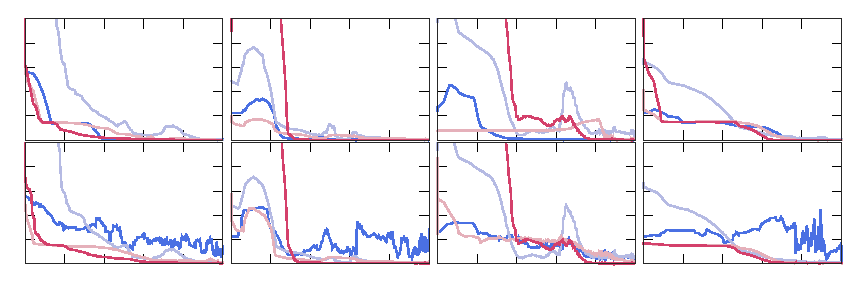
\includegraphics{./figures/parts/02/chapters/04/sections/04/smsm_max_range_limitations_1}}%
    \gplfronttext
  \end{picture}%
\endgroup
